\textbf{Входные параметры:}
 
Parameters --- Вектор параметров генетического алгоритма. Каждый элемент обозначает свой параметр:
 
 \begin{itemize}
 \item [0] --- длина бинарной хромосомы (определяется задачей оптимизации, что мы решаем);
 
 \item [1] --- число вычислений целевой функции (CountOfFitness);
 
 \item [2] --- тип селекции (TypeOfSel):
 
 \begin{itemize}
       \item 0 --- ProportionalSelection (Пропорциональная селекция);
 
       \item 1 --- RankSelection (Ранговая селекция);
 
       \item 2 --- TournamentSelection (Турнирная селекция).
	    \end{itemize}
 
 \item [3] --- тип скрещивания (TypeOfCros):
  \begin{itemize}
       \item 0 --- SinglepointCrossover (Одноточечное скрещивание);
 
       \item 1 --- TwopointCrossover (Двухточечное скрещивание);
 
       \item 2 --- UniformCrossover (Равномерное скрещивание).
	    \end{itemize}
 
 \item [4] --- тип мутации (TypeOfMutation):
  \begin{itemize}
       \item 0 --- Weak (Слабая мутация);
 
       \item 1 --- Average (Средняя мутация);
 
       \item 2 --- Strong (Сильная мутация).
	    \end{itemize}
 
 \item [5] --- тип формирования нового поколения (TypeOfForm):
  \begin{itemize}
       \item 0 --- OnlyOffspringGenerationForming (Только потомки);
 
       \item 1 --- OnlyOffspringWithBestGenerationForming (Только потомки и копия лучшего индивида).
	    \end{itemize}
 \end{itemize}
 
FitnessFunction --- указатель на целевую функцию (если решается задача условной оптимизации, то учет ограничений должен быть включен в эту функцию);
 
VHML\_ResultVector --- найденное решение (бинарный вектор);
 
VHML\_Result --- значение целевой функции в точке, определенной вектором VHML\_ResultVector.

\textbf{Возвращаемое значение:} 

 1 --- завершил работу без ошибок. Всё хорошо.
 
 0 --- возникли при работе ошибки. Скорее всего в этом случае в VHML\_ResultVector и в VHML\_Result не содержится решение задачи.

 \textbf{Принцип работы} смотрите ниже на рисунке \ref{img:HML_StandartBinaryGeneticAlgorithm_Sheme} на странице \pageref{img:HML_StandartBinaryGeneticAlgorithm_Sheme}.

\begin{figure} [h]
  \center
  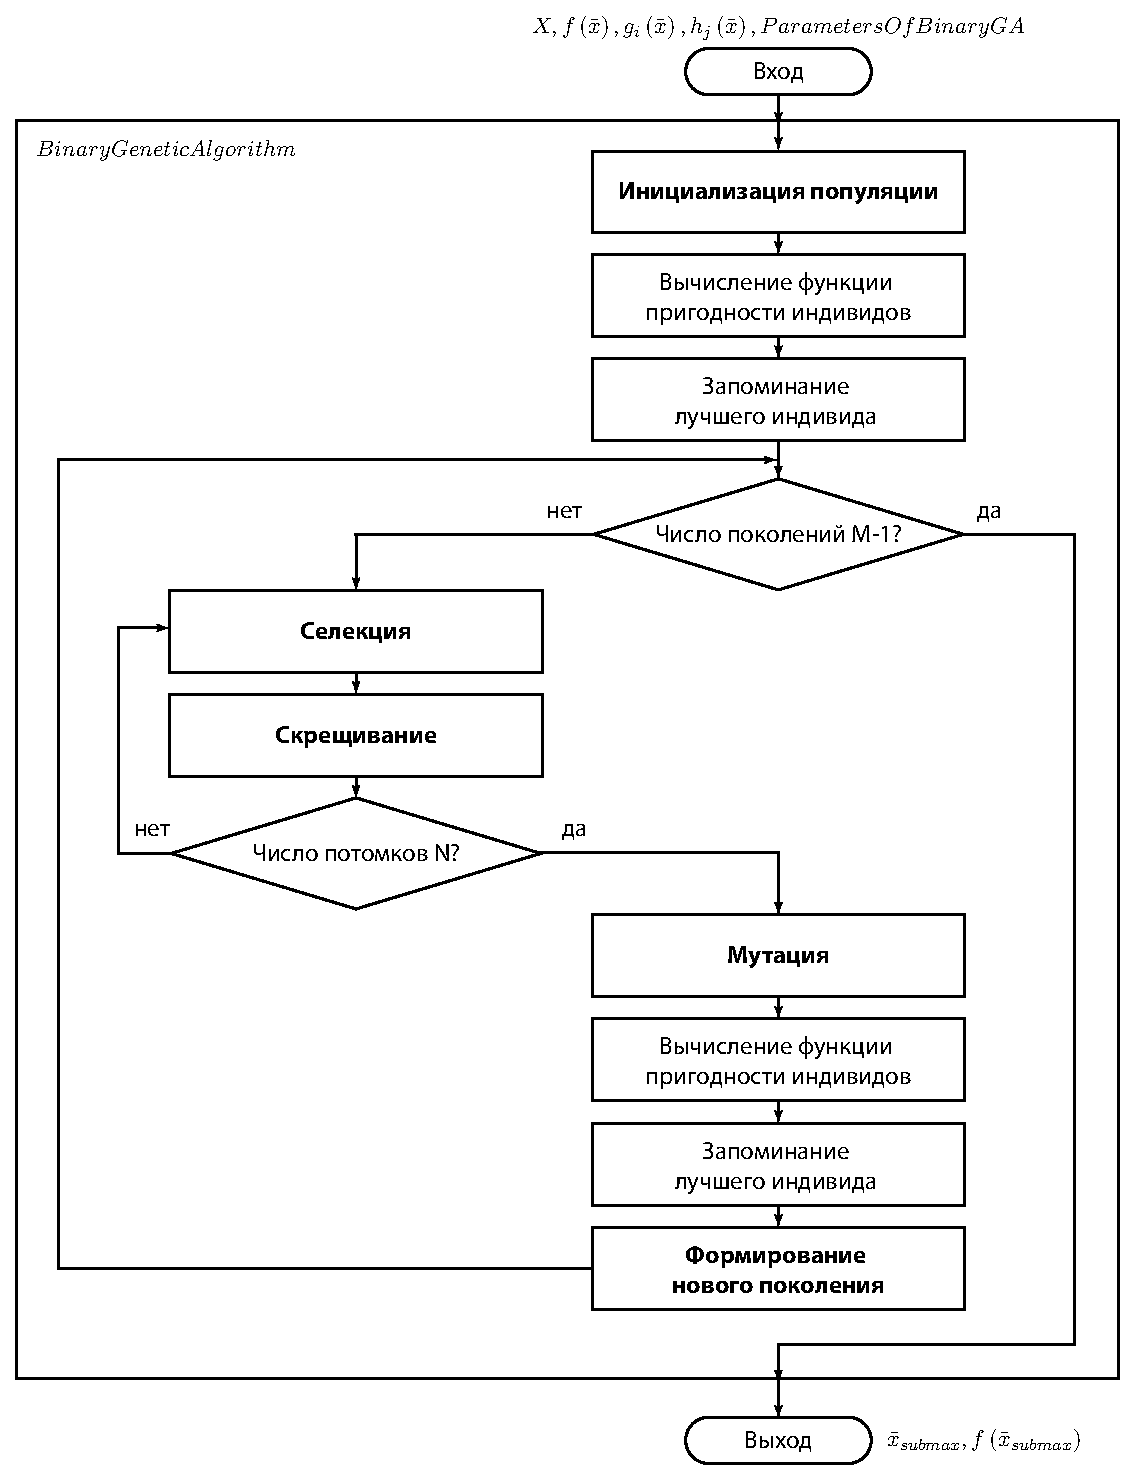
\includegraphics [scale=0.5] {HML_StandartBinaryGeneticAlgorithm_Sheme}
  \caption{Механизм работы генетического алгоритма} 
  \label{img:HML_StandartBinaryGeneticAlgorithm_Sheme}  
\end{figure}

\textbf{О функции:}

Реализация алгоритма из документа <<Генетический алгоритм. Стандарт. v.3.0>>.

\href{https://github.com/Harrix/Standard-Genetic-Algorithm}{https://github.com/Harrix/Standard-Genetic-Algorithm}

Алгоритм бинарной оптимизации. Ищет максимум целевой функции FitnessFunction.

Решением является бинарная строка, то есть вектор, состоящий из 0 и 1.

\textbf{Примерный настройки} (для примера Вы можете поставить такие рабочие настройки):

 Parameters[0]=50;
 
Parameters[1]=100*100;

Parameters[2]=2;

Parameters[3]=2;

Parameters[4]=1;

Parameters[5]=1;


\textbf{Примечание:}

 На рисунке блок-схемы сГА на бинарных строках число поколений обозначено буквой \textbf{M}, в коде функции же обозначается переменной \textbf{NumberOfGenerations}.


\textbf{Примечание:}

 В сГА на бинарных строках не нужно задавать в параметрах число поколений и размер популяции, а только число вычислений целевой функции. Почему? Алгоритм сам определит число поколений и размер популяции, исходя из принципа, что число поколений и размер популяции должны быть примерно равны. Поэтому выбирайте значение Parameters[1] в виде:

int K=100;

Parameters[1]=K*K;

То есть в виде квадрата целого числа. В противном случае реальное число вычислений целевой функции и значение Parameters[1] будут не совпадать.

Код целевой функции:
\begin{lstlisting}[caption=Оптимизируемая функция]
double Func(int *x,int VHML_N)
{
//Сумма всех элементов массива
return HML_SumVector(x,VHML_N);
}
//---------------------------------------------------------------------------
\end{lstlisting}